\documentclass[paper=a4, fontsize=11pt]{scrartcl} % A4 paper and 11pt font size
\usepackage[utf8]{inputenc}

\usepackage[T1]{fontenc} % Use 8-bit encoding that has 256 glyphs
\usepackage[ngerman]{babel} % English language/hyphenation
\usepackage{amsmath,amsfonts,amsthm} % Math packages

\usepackage{graphicx}
\usepackage{float}

\usepackage{sectsty} % Allows customizing section commands
\allsectionsfont{\centering \normalfont\scshape} % Make all sections centered, the default font and small caps

\usepackage{fancyhdr} % Custom headers and footers
\pagestyle{fancyplain} % Makes all pages in the document conform to the custom headers and footers
\fancyhead{} % No page header - if you want one, create it in the same way as the footers below
\fancyfoot[L]{} % Empty left footer
\fancyfoot[C]{} % Empty center footer
\fancyfoot[R]{\thepage} % Page numbering for right footer
\renewcommand{\headrulewidth}{0pt} % Remove header underlines
\renewcommand{\footrulewidth}{0pt} % Remove footer underlines
\setlength{\headheight}{13.6pt} % Customize the height of the header

\numberwithin{equation}{section} % Number equations within sections (i.e. 1.1, 1.2, 2.1, 2.2 instead of 1, 2, 3, 4)
\numberwithin{figure}{section} % Number figures within sections (i.e. 1.1, 1.2, 2.1, 2.2 instead of 1, 2, 3, 4)
\numberwithin{table}{section} % Number tables within sections (i.e. 1.1, 1.2, 2.1, 2.2 instead of 1, 2, 3, 4)

\setlength\parindent{0pt} % Removes all indentation from paragraphs - comment this line for an assignment with lots of text

\newcommand {\horrule}[1]{\rule{\linewidth}{#1}} % Create horizontal rule command with 1 argument of height

\title {
  \normalfont \normalsize
  \textsc{HAW Hamburg} \\ [25pt] % Your university, school and/or department name(s)
  \textsc{Technik und Technologie von vernetzen Systeme} \\ [15pt]
  \horrule{0.5pt} \\[0.4cm] % Thin top horizontal rule
  \huge LoWPAN Networking im IoT \\ [15pt] % The assignment title
  \small Prof. Dr. Fohl \\
  \horrule{2pt} \\[0.5cm] % Thick bottom horizontal rule
}

\author{Fabien Lapok, Matthias Nitsche}

\date{\normalsize\today}

\begin{document}

\maketitle

\section{Aufgabe - Laboreinbindung von Gateways und Sensorknoten}

Nach dem Aufsetzen von Szenario 1 haben wir mit Wireshark - siehe Abbildung \ref{fig:hrwireshark} - die Neighbor Discovery von Host zu Router mitgeschnitten.

\begin{figure}[H]
  \centering
  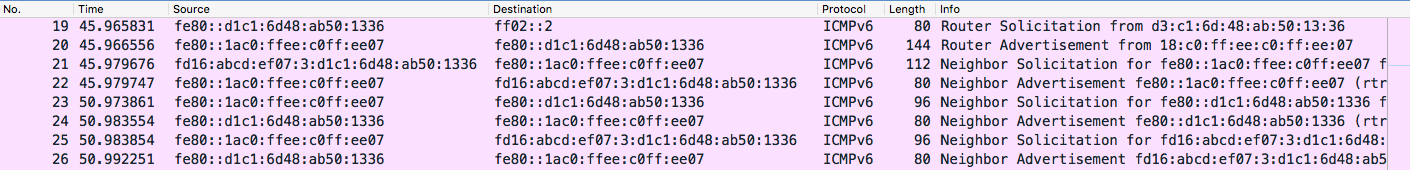
\includegraphics[width=\linewidth]{imgs/host-to-router-interaction-wireshark.png}
  \caption{Host zu Router Interaktion Wireshark Mitschnitt}
  \label{fig:hrwireshark}
\end{figure}

Der Ablauf des Protokolls ist detailliert in RFC 6775 ``''Neighbor Discovery Optimization``'' unter Host-to-Router interaction beschrieben. In Abbildung \ref{fig:hrfluss} ist ein Flussdiagramm was den Austausch vom Raspberry Pi (RPI) als Rouer zum Sensor als Host beschreibt.
\\
\\
Die ersten 4 Schritte laufen Ordnungsgemäß wie in RFC 6775 ab. Sensor fragt nach Router ``Router Solicitation'', RPI antwortet ``Router Advertisment'', Sensor fragt Router nach der Nachbarschaft ``Neighbor Solicitation'' und RPI antwortet mit ``Neighbor Advertisement''. Nach 5 Sekunden wird die Nachbarschaftsanfrage erneut gesendet.

\begin{figure}[H]
  \centering
  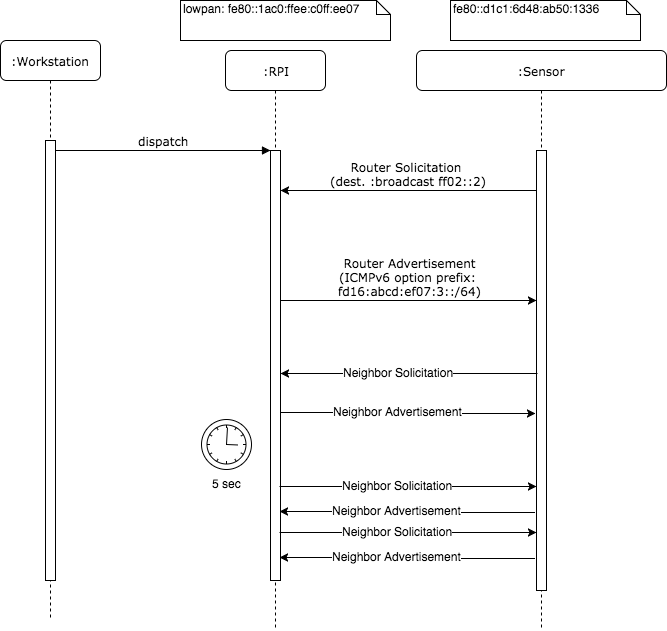
\includegraphics[width=0.7\linewidth,height=0.7\columnwidth]{imgs/host-to-router-interaction.png}
  \caption{Host zu Router Interaktion Flussdiagramm}
  \label{fig:hrfluss}
\end{figure}

Uns sind keine Auffälligkeiten im Vergleich zum RFC 6775 aufgefallen.

\section{Aufgabe - RPL Routing im Labornetz}

Some text...

\section{Aufgabe - Datenverteilung und Messung}

Im folgenden machen wir mittels COAP, HTTP ähnliche Anfragen um die REST Ressourcen auf den (RIOT) Sensoren auszulesen. Wir haben die ``led'' mittels ``PUT 1'' und ``PUT 0'' an verschiedenen Rechnern an und ausgeschaltet sowie ``temperature'' und ``humidity'' ausgelesen. Wie zuvor wurde die Kommunikation über Wireshark aufgezeichnet.

\subsection{Messung}

Vorgehen?... haha .. Vorgehen :( - Welche Rechner? Welche Standorte? etc.

\paragraph{Paketverlust}

Paketverlust text..

\begin{figure}[H]
  \centering
  \includegraphics[width=0.7\linewidth,height=0.7\columnwidth]{imgs/paketverlust.png}
  \caption{Paketverlust nach Reihe (e.g. Root vs 1. vs 2.)}
  \label{fig:paketverlust}
\end{figure}

\paragraph{Sendedauer}

Sendedauer text..

\begin{figure}[H]
  \centering
  \includegraphics[width=0.7\linewidth,height=0.7\columnwidth]{imgs/sendedauer.png}
  \caption{Mittlere Sendedauer (Balken oder Sequenzdiagramm)}
  \label{fig:sendedauer}
\end{figure}

\end{document}

